\documentclass[aspectratio=169,11pt]{beamer}

% =========================================================
% Theme
% =========================================================
\usetheme{Madrid}
\usecolortheme{seahorse}
\setbeamertemplate{navigation symbols}{}

% =========================================================
% Packages
% =========================================================
\usepackage[utf8]{inputenc}
\usepackage[T1]{fontenc}
\usepackage{lmodern}
\usepackage{amsmath,amssymb}
\usepackage{xcolor}
\usepackage{booktabs}
\usepackage{array}
\usepackage{listings}
\usepackage{tikz}
\usetikzlibrary{arrows.meta,positioning,fit,calc,shapes.geometric}
\usepackage{hyperref}
\hypersetup{pdfpagemode=UseNone}

% =========================================================
% Colors
% =========================================================
\definecolor{deepblue}{RGB}{0,51,102}
\definecolor{softblue}{RGB}{220,235,247}
\definecolor{softgreen}{RGB}{223,242,228}
\definecolor{softorange}{RGB}{255,238,214}
\definecolor{softred}{RGB}{252,228,228}
\definecolor{codebg}{RGB}{248,248,248}
\definecolor{mygray}{RGB}{90,90,90}
\definecolor{mypurple}{RGB}{102,0,153}

% =========================================================
% Listings
% =========================================================
\lstset{
	language=Java,
	basicstyle=\ttfamily\small,
	backgroundcolor=\color{codebg},
	frame=single,
	breaklines=true,
	columns=fullflexible,
	showstringspaces=false,
	keywordstyle=\color{deepblue}\bfseries,
	commentstyle=\color{green!50!black},
	stringstyle=\color{mypurple},
	numbers=left,
	numberstyle=\tiny\color{mygray},
	stepnumber=1,
	numbersep=8pt
}

% =========================================================
% Title Info
% =========================================================
\title[Week 4 -- Part 1]{Concurrency and Distributed Systems}
\subtitle{Week 4 -- Part 1: Java Memory Model and Visibility}
\author{Dr. Mohamad Aoude}
\institute{Faculty of Engineering}
\date{\today}

% =========================================================
% Custom Blocks
% =========================================================
\setbeamercolor{block title}{bg=deepblue!85, fg=white}
\setbeamercolor{block body}{bg=softblue, fg=black}

\setbeamercolor{alertblock title}{bg=red!75!black, fg=white}
\setbeamercolor{alertblock body}{bg=softred, fg=black}

\setbeamercolor{exampleblock title}{bg=green!50!black, fg=white}
\setbeamercolor{exampleblock body}{bg=softgreen, fg=black}

% =========================================================
% Footer
% =========================================================
\setbeamertemplate{footline}{
	\leavevmode
	\hbox{
		\begin{beamercolorbox}[wd=.78\paperwidth,ht=2.5ex,dp=1.2ex,leftskip=0.3cm]{author in head/foot}
			\usebeamerfont{author in head/foot}Concurrency and Distributed Systems --- Week 4 Part 1
		\end{beamercolorbox}
		\begin{beamercolorbox}[wd=.22\paperwidth,ht=2.5ex,dp=1.2ex,rightskip=0.3cm]{date in head/foot}
			\hfill \insertframenumber/\inserttotalframenumber
		\end{beamercolorbox}
	}
}

% =========================================================
% Document
% =========================================================
\begin{document}
	
	% =========================================================
	\begin{frame}
		\titlepage
	\end{frame}
	
	% =========================================================
	\begin{frame}{Part 1 Roadmap}
		\tableofcontents
	\end{frame}
	
	\section{Why Memory Visibility Matters}
	\section{The Stop-Flag Problem}
	\section{Hardware Intuition}
	\section{Java Memory Model}
	\section{Data Races}
	\section{Engineering Takeaways}
	\section{Lab Preparation}
	
	% =========================================================
	\begin{frame}{Why This Part Matters}
		\begin{block}{Core question}
			When one thread writes a value, \textbf{when} does another thread see it?
		\end{block}
		
		\vspace{0.3cm}
		
		In sequential programming, this question barely appears.  
		In concurrent programming, it is one of the central correctness questions.
		
		\vspace{0.3cm}
		
		\begin{itemize}
			\item A program may look logically correct
			\item The variable may truly be updated
			\item Yet another thread may continue seeing an older value
		\end{itemize}
		
		\vspace{0.3cm}
		
		\begin{alertblock}{Main message}
			Concurrency is not only about \textbf{multiple threads running}.  
			It is also about \textbf{what each thread is allowed to observe}.
		\end{alertblock}
	\end{frame}
	
	% =========================================================
	\begin{frame}{From Week 3 to Week 4}
		\begin{block}{Week 3}
			We studied mechanisms that control \textbf{entry into critical sections}:
			\begin{itemize}
				\item \texttt{synchronized}
				\item \texttt{ReentrantLock}
			\end{itemize}
		\end{block}
		
		\vspace{0.25cm}
		
		\begin{block}{Week 4}
			Now we study the memory side of concurrency:
			\begin{itemize}
				\item visibility
				\item ordering
				\item the Java Memory Model
				\item why stale reads happen
				\item why visibility is different from atomicity
			\end{itemize}
		\end{block}
		
		\vspace{0.25cm}
		
		\begin{exampleblock}{Pedagogical transition}
			Week 3 asked: \emph{Who is allowed to enter?}
			
			Week 4 asks: \emph{What is each thread allowed to see?}
		\end{exampleblock}
	\end{frame}
	
	% =========================================================
	\begin{frame}{Learning Objectives}
		By the end of this lecture, students should be able to:
		
		\begin{itemize}
			\item explain why stale reads can happen
			\item describe, informally, the role of caches, registers, and reordering
			\item explain why Java needs a formal memory model
			\item distinguish between:
			\begin{itemize}
				\item computation correctness in one thread
				\item observation correctness across threads
			\end{itemize}
			\item define \textbf{visibility} in practical terms
			\item identify an informal \textbf{data race}
			\item prepare for the use of \texttt{volatile} in the next lecture
		\end{itemize}
	\end{frame}
	
	% =========================================================
	\begin{frame}{The Naive Mental Model}
		Many students initially imagine shared memory like this:
		
		\vspace{0.2cm}
		\centering
		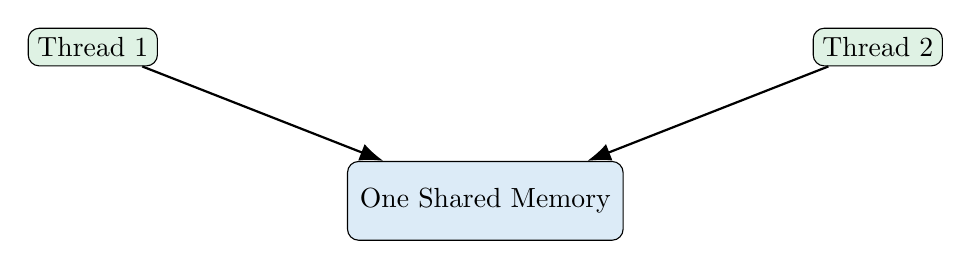
\begin{tikzpicture}[node distance=1.7cm]
			\node[draw, rounded corners, fill=softblue, minimum width=3.5cm, minimum height=1cm] (mem) {One Shared Memory};
			\node[draw, rounded corners, fill=softgreen, above left=1.2cm and 2.4cm of mem] (t1) {Thread 1};
			\node[draw, rounded corners, fill=softgreen, above right=1.2cm and 2.4cm of mem] (t2) {Thread 2};
			
			\draw[-{Latex[length=3mm]}, thick] (t1) -- (mem);
			\draw[-{Latex[length=3mm]}, thick] (t2) -- (mem);
		\end{tikzpicture}
		
		\vspace{0.4cm}
		
		\begin{block}{Naive assumption}
			Every read goes directly to shared memory, and every write is instantly visible to everyone.
		\end{block}
		
		\begin{alertblock}{Problem}
			That is not how modern concurrent execution should be mentally modeled.
		\end{alertblock}
	\end{frame}
	
	% =========================================================
	\begin{frame}{The Real System Is More Complicated}
		A more realistic picture includes multiple layers:
		
		\vspace{0.2cm}
		\centering
		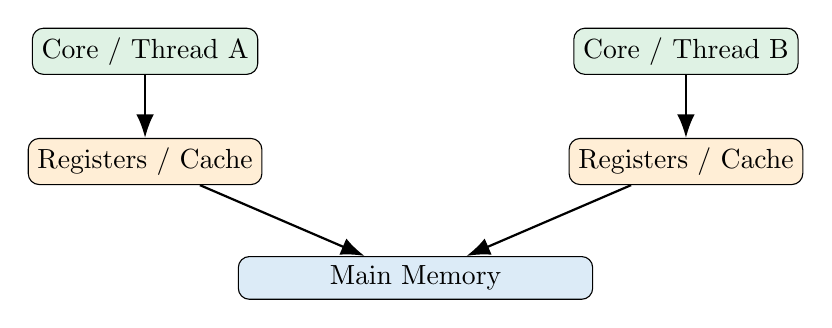
\begin{tikzpicture}[node distance=0.8cm and 1.2cm]
			\node[draw, rounded corners, fill=softgreen, minimum width=2.3cm] (core1) {Core / Thread A};
			\node[draw, rounded corners, fill=softgreen, right=4cm of core1, minimum width=2.3cm] (core2) {Core / Thread B};
			
			\node[draw, rounded corners, fill=softorange, below=of core1, minimum width=2.3cm] (cache1) {Registers / Cache};
			\node[draw, rounded corners, fill=softorange, below=of core2, minimum width=2.3cm] (cache2) {Registers / Cache};
			
			\node[draw, rounded corners, fill=softblue, below=1.2cm of $(cache1)!0.5!(cache2)$, minimum width=4.5cm] (memory) {Main Memory};
			
			\draw[-{Latex[length=3mm]}, thick] (core1) -- (cache1);
			\draw[-{Latex[length=3mm]}, thick] (core2) -- (cache2);
			\draw[-{Latex[length=3mm]}, thick] (cache1) -- (memory);
			\draw[-{Latex[length=3mm]}, thick] (cache2) -- (memory);
		\end{tikzpicture}
		
		\vspace{0.4cm}
		
		\begin{itemize}
			\item values may be cached
			\item values may stay in registers
			\item reads may not observe the latest write immediately
			\item compiler and CPU may reorder operations
		\end{itemize}
	\end{frame}
	
	% =========================================================
	\begin{frame}[fragile]{First Contradiction: The Stop-Flag Example}
		\begin{lstlisting}
			class StopDemo {
				static boolean running = true;
				
				public static void main(String[] args) throws Exception {
					Thread worker = new Thread(() -> {
						while (running) {
							// busy wait
						}
						System.out.println("Worker stopped");
					});
					
					worker.start();
					
					Thread.sleep(1000);
					running = false;
					System.out.println("Main changed running = false");
				}
			}
		\end{lstlisting}
	\end{frame}
	
	% =========================================================
	\begin{frame}{Question: Why Might This Fail?}
		At first glance, the code seems simple:
		
		\begin{itemize}
			\item main thread writes \texttt{running = false}
			\item worker thread repeatedly checks \texttt{running}
			\item therefore the worker should stop
		\end{itemize}
		
		\vspace{0.3cm}
		
		\begin{alertblock}{But in concurrent execution}
			The worker may keep seeing an older value, such as \texttt{true}.
		\end{alertblock}
		
		\vspace{0.3cm}
		
		Possible reasons include:
		\begin{itemize}
			\item cached value reused
			\item value kept in register
			\item lack of synchronization semantics
			\item legal compiler/runtime optimizations
		\end{itemize}
		
		\vspace{0.3cm}
		
		\begin{exampleblock}{Important insight}
			The variable may have changed in one thread, but that does \emph{not} automatically mean another thread must observe the change immediately.
		\end{exampleblock}
	\end{frame}
	
	% =========================================================
	\begin{frame}{Visibility: Informal Definition}
		\begin{block}{Visibility}
			Visibility asks whether a write performed by one thread becomes observable by another thread.
		\end{block}
		
		\vspace{0.3cm}
		
		\begin{center}
			\begin{tabular}{>{\bfseries}m{3cm} m{7.5cm}}
				Write correctness & Was the value updated at all? \\
				Observation correctness & Did the other thread actually see that update? \\
			\end{tabular}
		\end{center}
		
		\vspace{0.3cm}
		
		\begin{alertblock}{Concurrency reality}
			A value can be correctly written, yet still not be promptly visible to another thread.
		\end{alertblock}
	\end{frame}
	
	% =========================================================
	\begin{frame}{Engineering Intuition: Why Hardware Does This}
		Why are processors designed this way?
		
		\begin{itemize}
			\item accessing memory is expensive
			\item caches reduce latency
			\item registers reduce repeated loads
			\item CPUs reorder internally for performance
			\item compilers optimize aggressively when semantics allow it
		\end{itemize}
		
		\vspace{0.3cm}
		
		\begin{block}{Performance principle}
			Modern systems are optimized for throughput and efficiency, not for a naive line-by-line human mental model.
		\end{block}
		
		\vspace{0.3cm}
		
		\begin{alertblock}{Key takeaway}
			Concurrency correctness requires \textbf{explicit memory semantics}.  
			It cannot rely on intuition alone.
		\end{alertblock}
	\end{frame}
	
	% =========================================================
	\begin{frame}{Single-Thread Semantics vs Multi-Thread Observation}
		\begin{columns}[T]
			\column{0.48\textwidth}
			\begin{block}{Single-thread view}
				If a compiler reorders operations but preserves the meaning for one thread, the transformation may be allowed.
			\end{block}
			
			\column{0.48\textwidth}
			\begin{block}{Multi-thread view}
				That same reordering may affect what another thread can observe, unless synchronization rules forbid it.
			\end{block}
		\end{columns}
		
		\vspace{0.35cm}
		
		\begin{exampleblock}{Important distinction}
			An optimization may be harmless for one thread but dangerous for shared-memory reasoning across threads.
		\end{exampleblock}
		
		\vspace{0.25cm}
		
		\begin{alertblock}{This is why a formal memory model is necessary}
			Without it, developers would have no stable basis for reasoning about concurrent code.
		\end{alertblock}
	\end{frame}
	
	% =========================================================
	\begin{frame}{A More Realistic Observation Timeline}
		\centering
		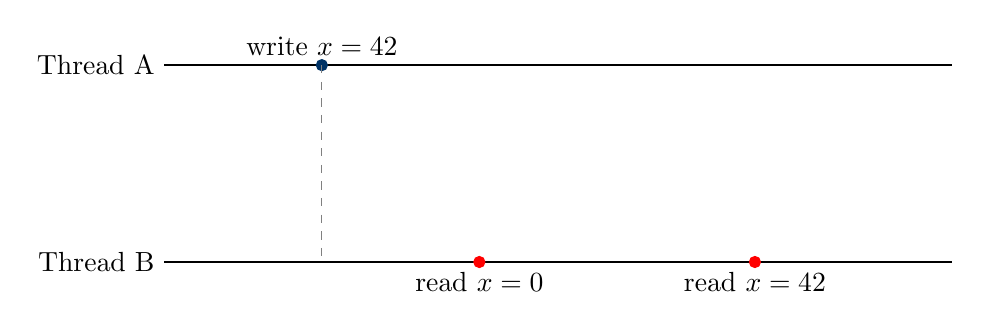
\begin{tikzpicture}[x=1cm,y=1cm]
			% timeline A
			\draw[thick] (0,4) -- (10,4);
			\node[left] at (0,4) {Thread A};
			
			% timeline B
			\draw[thick] (0,1.5) -- (10,1.5);
			\node[left] at (0,1.5) {Thread B};
			
			% events A
			\filldraw[deepblue] (2,4) circle (2pt);
			\node[above] at (2,4) {write $x=42$};
			
			% events B
			\filldraw[red] (4,1.5) circle (2pt);
			\node[below] at (4,1.5) {read $x=0$};
			
			\filldraw[red] (7.5,1.5) circle (2pt);
			\node[below] at (7.5,1.5) {read $x=42$};
			
			\draw[dashed, gray] (2,4) -- (2,1.5);
		\end{tikzpicture}
		
		\vspace{0.4cm}
		
		\begin{block}{What this means}
			Even after Thread A writes a new value, Thread B may not immediately observe that value in unsynchronized code.
		\end{block}
		
		\begin{alertblock}{Do not assume}
			\texttt{write now} does \emph{not} imply \texttt{everyone sees it now}.
		\end{alertblock}
	\end{frame}
	
	% =========================================================
	\begin{frame}{The Java Memory Model (JMM)}
		\begin{block}{Definition}
			The Java Memory Model is the formal specification that defines how threads interact through memory in Java.
		\end{block}
		
		\vspace{0.3cm}
		
		It provides rules about:
		\begin{itemize}
			\item what values reads are allowed to see
			\item when writes become visible
			\item which reorderings are legal
			\item how synchronization establishes guarantees
		\end{itemize}
		
		\vspace{0.3cm}
		
		\begin{exampleblock}{Why it matters}
			The JMM is the bridge between:
			\begin{itemize}
				\item Java source code
				\item compiler / JIT optimizations
				\item hardware execution realities
			\end{itemize}
		\end{exampleblock}
	\end{frame}
	
	% =========================================================
	\begin{frame}{Why Java Needs a Memory Model}
		Without a formal memory model:
		
		\begin{itemize}
			\item every processor could behave differently
			\item every JVM optimization could break assumptions differently
			\item concurrent code would become non-portable and non-reasonable
		\end{itemize}
		
		\vspace{0.3cm}
		
		\begin{alertblock}{Practical answer}
			The JMM gives developers a contract:
			\begin{quote}
				If you use the right synchronization constructs, Java guarantees certain visibility and ordering properties.
			\end{quote}
		\end{alertblock}
		
		\vspace{0.25cm}
		
		\begin{block}{Practical engineering viewpoint}
			The JMM does not promise “intuitive behavior.”  
			It promises \textbf{defined behavior}.
		\end{block}
	\end{frame}
	
	% =========================================================
	\begin{frame}{What This Lecture Covers vs Later Parts}
		\centering
		\begin{tabular}{>{\bfseries}m{3.2cm} m{7.6cm}}
			Part 1 & Why stale reads and visibility problems exist \\
			Part 2 & \texttt{volatile} and happens-before \\
			Part 3 & Visibility vs atomicity; broken DCL \\
			Part 4 & \texttt{AtomicInteger}, CAS, contention \\
		\end{tabular}
		
		\vspace{0.45cm}
		
		\begin{exampleblock}{Pedagogical logic}
			Before students can use \texttt{volatile}, they must first understand \emph{why} unsynchronized code can fail.
		\end{exampleblock}
	\end{frame}
	
	% =========================================================
	\begin{frame}{Informal Data Race Idea}
		\begin{block}{Informal definition}
			A data race occurs when:
			\begin{itemize}
				\item two or more threads access the same variable
				\item at least one access is a write
				\item there is no proper synchronization establishing safe ordering / visibility
			\end{itemize}
		\end{block}
		
		\vspace{0.3cm}
		
		\begin{alertblock}{Why data races matter}
			Once shared access is unsafely concurrent, behavior becomes much harder to reason about.
		\end{alertblock}
		
		\vspace{0.25cm}
		
		\begin{exampleblock}{Important nuance}
			A data race is not just “two threads touching the same variable.”  
			It is unsafely touching it without the needed memory guarantees.
		\end{exampleblock}
	\end{frame}
	
	% =========================================================
	\begin{frame}[fragile]{StopDemo as an Informal Data Race Example}
		\begin{lstlisting}
			static boolean running = true;
		\end{lstlisting}
		
		Two threads access \texttt{running}:
		
		\begin{itemize}
			\item Thread A writes \texttt{running = false}
			\item Thread B repeatedly reads \texttt{running}
		\end{itemize}
		
		\vspace{0.3cm}
		
		There is no:
		\begin{itemize}
			\item \texttt{volatile}
			\item monitor synchronization
			\item explicit lock-based communication
		\end{itemize}
		
		\vspace{0.3cm}
		
		\begin{alertblock}{Conclusion}
			This is an unsafely shared variable communication pattern.  
			It is exactly the kind of situation where stale reads may appear.
		\end{alertblock}
	\end{frame}
	
	% =========================================================
	\begin{frame}[fragile]{Why Adding \texttt{println} Can Change Behavior}
		A classic student surprise is this:
		
		\begin{lstlisting}
			while (running) {
				System.out.println("still running...");
			}
		\end{lstlisting}
		
		Now the program may appear to ``work better.''
		
		\vspace{0.3cm}
		
		\begin{block}{Why?}
			Because adding logging changes:
			\begin{itemize}
				\item timing
				\item scheduling
				\item optimization opportunities
				\item possibly synchronization side effects inside library code
			\end{itemize}
		\end{block}
		
		\vspace{0.25cm}
		
		\begin{alertblock}{Critical lesson}
			When a concurrency bug disappears after adding output, the bug is usually \textbf{masked}, not solved.
		\end{alertblock}
	\end{frame}
	
	% =========================================================
	\begin{frame}{Debugging Trap: Observation Can Disturb the System}
		\begin{center}
			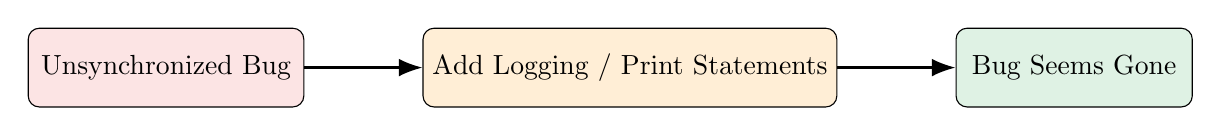
\begin{tikzpicture}[node distance=1cm]
				\node[draw, rounded corners, fill=softred, minimum width=3.5cm, minimum height=1cm] (bug) {Unsynchronized Bug};
				\node[draw, rounded corners, fill=softorange, right=1.5cm of bug, minimum width=3.6cm, minimum height=1cm] (log) {Add Logging / Print Statements};
				\node[draw, rounded corners, fill=softgreen, right=1.5cm of log, minimum width=3cm, minimum height=1cm] (mask) {Bug Seems Gone};
				
				\draw[-{Latex[length=3mm]}, thick] (bug) -- (log);
				\draw[-{Latex[length=3mm]}, thick] (log) -- (mask);
			\end{tikzpicture}
		\end{center}
		
		\vspace{0.35cm}
		
		\begin{exampleblock}{Engineering reality}
			Concurrency bugs are often:
			\begin{itemize}
				\item timing-sensitive
				\item schedule-dependent
				\item sensitive to instrumentation
			\end{itemize}
		\end{exampleblock}
		
		\vspace{0.25cm}
		
		\begin{alertblock}{Implication}
			Never conclude “it is fixed” just because it stops failing under observation.
		\end{alertblock}
	\end{frame}
	
	% =========================================================
	\begin{frame}{Visibility Is Not the Same as Atomicity}
		This lecture is about \textbf{visibility}, but students must already see the boundary.
		
		\vspace{0.3cm}
		
		\begin{columns}[T]
			\column{0.48\textwidth}
			\begin{block}{Visibility}
				Did one thread see another thread's update?
			\end{block}
			
			\column{0.48\textwidth}
			\begin{block}{Atomicity}
				Did a multi-step operation behave as one indivisible action?
			\end{block}
		\end{columns}
		
		\vspace{0.35cm}
		
		\begin{exampleblock}{Why preview this now?}
			Students often confuse:
			\begin{itemize}
				\item ``I can see the latest value''
				\item with
				\item ``my update is thread-safe''
			\end{itemize}
		\end{exampleblock}
		
		\vspace{0.2cm}
		
		Part 2 and Part 3 will separate these carefully.
	\end{frame}
	
	% =========================================================
	\begin{frame}{Three Core Questions of Shared Memory Concurrency}
		\begin{enumerate}
			\item \textbf{Visibility:}  
			Can one thread see what another thread wrote?
			
			\vspace{0.15cm}
			\item \textbf{Ordering:}  
			Are operations observed in the required order?
			
			\vspace{0.15cm}
			\item \textbf{Atomicity:}  
			Does a multi-step update behave as one unit?
		\end{enumerate}
		
		\vspace{0.35cm}
		
		\begin{block}{Week 4 structure}
			\begin{itemize}
				\item Part 1 emphasizes visibility intuition
				\item Part 2 introduces visibility + ordering with \texttt{volatile}
				\item Part 3 addresses atomicity and DCL
				\item Part 4 introduces atomics and CAS
			\end{itemize}
		\end{block}
	\end{frame}
	
	% =========================================================
	\begin{frame}{A Practical Mental Model for Students}
		When reasoning about unsynchronized shared variables, do \emph{not} assume:
		
		\begin{itemize}
			\item every read gets the newest global value
			\item every write becomes instantly visible to all threads
			\item source code order is always the observation order across threads
		\end{itemize}
		
		\vspace{0.35cm}
		
		Instead, assume:
		
		\begin{itemize}
			\item threads may temporarily observe different views
			\item shared-memory communication requires proper semantics
			\item concurrency correctness must be deliberately engineered
		\end{itemize}
		
		\vspace{0.35cm}
		
		\begin{alertblock}{Good engineering posture}
			In concurrent code, \textbf{assume nothing is safely communicated unless the model guarantees it}.
		\end{alertblock}
	\end{frame}
	
	% =========================================================
	\begin{frame}{Mini Case Analysis}
		\begin{block}{Case}
			Thread A computes:
			\[
			done = true
			\]
			
			Thread B spins:
			\[
			\texttt{while (!done) \{ \}}
			\]
		\end{block}
		
		\vspace{0.25cm}
		
		\textbf{Question:} Why is this unsafe in plain shared-memory code?
		
		\vspace{0.25cm}
		
		\begin{exampleblock}{Reasoning}
			Because the program gives no formal memory-visibility guarantee that the spinning thread must observe the update promptly.
		\end{exampleblock}
		
		\vspace{0.25cm}
		
		\begin{alertblock}{This is the core of Part 1}
			The logic of the algorithm may be right, but the communication semantics are incomplete.
		\end{alertblock}
	\end{frame}
	
	% =========================================================
	\begin{frame}{What Students Should Stop Saying After This Lecture}
		After Part 1, students should stop saying:
		
		\begin{itemize}
			\item ``But I changed the variable, so the other thread must know''
			\item ``It works on my machine, so the memory behavior is correct''
			\item ``If the loop checks repeatedly, it will definitely see the new value''
			\item ``Adding print statements fixed the concurrency bug''
		\end{itemize}
		
		\vspace{0.35cm}
		
		\begin{alertblock}{Replace with}
			\begin{quote}
				Without explicit memory semantics, another thread may legally observe stale state.
			\end{quote}
		\end{alertblock}
	\end{frame}
	
	% =========================================================
	\begin{frame}{Concept Summary}
		\centering
		\begin{tabular}{>{\bfseries}m{3cm} m{7.5cm}}
			Visibility & whether one thread observes another thread's write \\
			Stale read & reading an older value after a newer one was written elsewhere \\
			JMM & Java's formal rules for memory interaction across threads \\
			Data race & unsafely concurrent access to shared data \\
			Key risk & code may look right but still communicate incorrectly \\
		\end{tabular}
	\end{frame}
	
	% =========================================================
	\begin{frame}{Lab Preparation for Part 1}
		\begin{block}{Lab 4.1 --- Stale Read Demo}
			Students run the stop-flag example and observe its behavior under different modifications.
		\end{block}
		
		\vspace{0.2cm}
		
		They should try:
		\begin{itemize}
			\item plain busy-wait loop
			\item adding \texttt{println}
			\item adding small work inside the loop
			\item repeating the run multiple times
		\end{itemize}
		
		\vspace{0.3cm}
		
		\textbf{Expected pedagogical outcome:}
		\begin{itemize}
			\item behavior is unstable
			\item debugging changes timing
			\item the root issue is lack of proper visibility guarantees
		\end{itemize}
	\end{frame}
	
	% =========================================================
	\begin{frame}{Discussion Questions}
		\begin{enumerate}
			\item Why is a shared variable not automatically a safe communication channel?
			\item Why can two threads temporarily observe different values?
			\item Why does adding output sometimes change concurrency behavior?
			\item What problem does the Java Memory Model solve?
			\item Why is stale visibility different from wrong arithmetic logic?
		\end{enumerate}
	\end{frame}
	
	% =========================================================
	\begin{frame}{Takeaway}
		\begin{alertblock}{Final takeaway for Part 1}
			In concurrent programming, correctness depends not only on what was written, but also on what other threads are allowed to see.
		\end{alertblock}
		
		\vspace{0.35cm}
		
		\begin{block}{Bridge to Part 2}
			Now that we understand \emph{why} stale reads happen, the next question becomes:
			
			\begin{center}
				\Large
				How do we force visibility and ordering guarantees in Java?
			\end{center}
		\end{block}
		
		\vspace{0.25cm}
		
		That leads directly to:
		\[
		\texttt{volatile} \quad \text{and} \quad \text{happens-before}
		\]
	\end{frame}
	
	% =========================================================
	\begin{frame}{End of Part 1}
		\centering
		\Huge Questions?
	\end{frame}
	
	% =========================================================
\end{document}